\documentclass[tikz,border=2pt]{standalone}
\usepackage{pgfplots}
\pgfplotsset{compat=1.18}
\usetikzlibrary{intersections}
\usepgfplotslibrary{fillbetween}

\begin{document}
	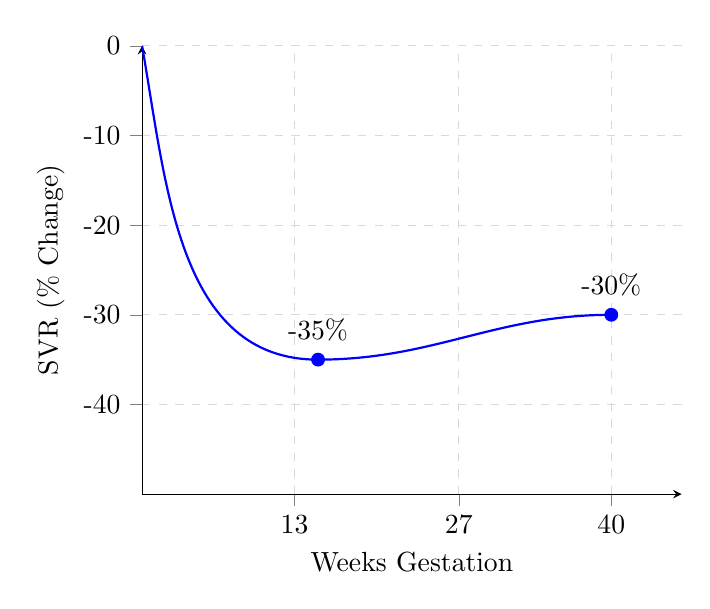
\begin{tikzpicture}
		\begin{axis}[
			axis lines=middle,
			ymin = 0,
			ymax = 50,
			xmin = 0,
			xmax= 46,
			grid = major,
			grid style={dashed, gray!30},
			ylabel near ticks,
			xlabel near ticks,
			xtick={13, 27, 40},
			xticklabels={13,27,40},
			yticklabels={,,-40,-30,-20,-10, 0},
			xlabel= Weeks Gestation,
			ylabel= SVR (\% Change),
			tick align=outside,
			legend pos= north east,
			legend style={font=\small, cells={align=left}}]

	
		\draw [blue, thick] (0,50) to [out = 280, in = 180] (15,15) node[circle,fill=blue,inner sep=0pt, label={[text = black]-35\%}, minimum size = 5pt]{} to [out = 0, in = 180] (40,20) node[circle,fill=blue,inner sep=0pt, label={[text = black]-30\%}, minimum size = 5pt]{};



%
		\end{axis}
	\end{tikzpicture} 
\end{document}